% NeST Policy 2: one-sparse neuron bridging (single-card figure).
\documentclass[tikz,border=8pt]{standalone}
\usepackage{amsmath,amssymb,bm}
\usetikzlibrary{positioning,calc}
\begin{document}
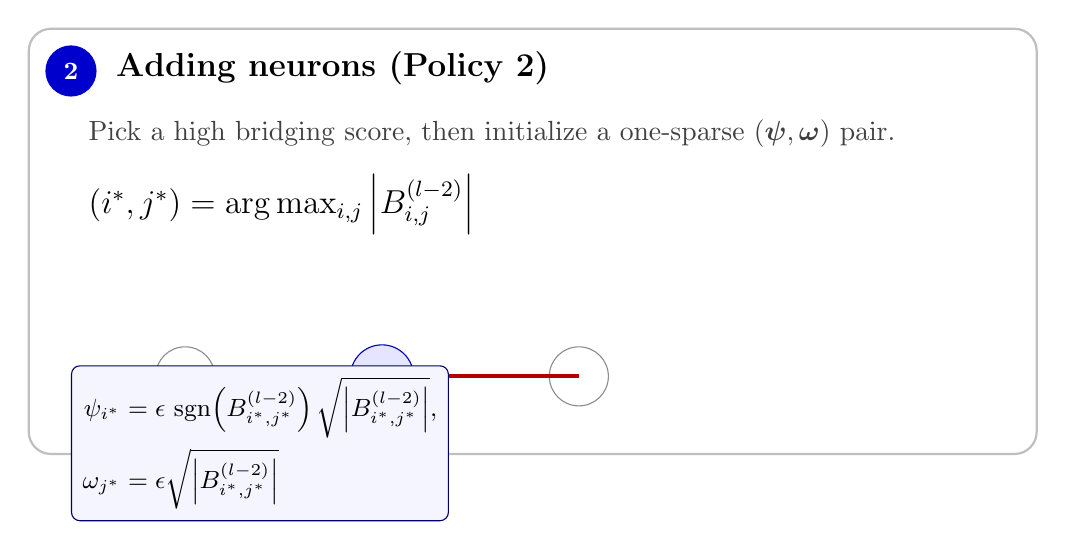
\begin{tikzpicture}[font=\sffamily]
\tikzset{
  card/.style={draw=black!25, rounded corners=8pt, fill=white, line width=0.8pt},
  nodec/.style={circle, draw=black!45, fill=white, minimum size=7.5mm, inner sep=0pt},
  newn/.style={circle, draw=blue!70!black, fill=blue!10, minimum size=8mm, inner sep=0pt},
  sel/.style={draw=red!70!black, line width=1.4pt},
  chip/.style={draw=blue!40!black, rounded corners=3pt, fill=blue!4, inner sep=3pt},
  stepnode/.style={circle, fill=blue!80!black, text=white, minimum size=6.5mm, inner sep=0pt, font=\bfseries\small}
}
\node[card, minimum width=12.8cm, minimum height=5.4cm, anchor=north west] (c) at (0,0) {};
\node[stepnode] at ($(c.north west)+(0.55,-0.55)$) {2};
\node[anchor=west, font=\bfseries\large] at ($(c.north west)+(1.0,-0.52)$) {Adding neurons (Policy~2)};
\node[anchor=west, font=\normalsize, text=black!75] at ($(c.north west)+(0.65,-1.35)$)
  {Pick a high bridging score, then initialize a one-sparse $(\bm{\psi},\bm{\omega})$ pair.};
\node[anchor=west, font=\large] at ($(c.north west)+(0.65,-2.25)$)
  {$(i^\ast,j^\ast)=\arg\max_{i,j}\left\lvert B^{(l-2)}_{i,j}\right\rvert$};
\coordinate (u) at ($(c.south west)+(2.0,1.0)$);
\coordinate (v) at ($(c.south west)+(4.5,1.0)$);
\coordinate (w) at ($(c.south west)+(7.0,1.0)$);
\node[nodec] at (u) {};
\node[newn] at (v) {};
\node[nodec] at (w) {};
\draw[sel] (u)--(v);
\draw[sel] (v)--(w);
\node[chip, anchor=west, font=\small, inner sep=4pt] at ($(c.south west)+(0.55,0.15)$)
{$\begin{aligned}
  \psi_{i^\ast} &= \epsilon\,\operatorname{sgn}\!\left(B^{(l-2)}_{i^\ast,j^\ast}\right)\sqrt{\left\lvert B^{(l-2)}_{i^\ast,j^\ast}\right\rvert},\\
  \omega_{j^\ast} &= \epsilon\sqrt{\left\lvert B^{(l-2)}_{i^\ast,j^\ast}\right\rvert}
\end{aligned}$};
\end{tikzpicture}
\end{document}
